%============================================================
%  Bookshop Automation System — Software Engineering Lab
%  Comprehensive Software Design Specification (SDS)
%  B.Tech Information Technology | VJTI Mumbai
%  Compile with: pdflatex -> pdflatex
%============================================================

\documentclass[12pt, a4paper]{report}

% ── Packages ────────────────────────────────────────────────
\usepackage[top=2.3cm, bottom=2.3cm, left=2.7cm, right=2.5cm]{geometry}
\usepackage{mathptmx}
\usepackage[T1]{fontenc}
\usepackage[utf8]{inputenc}
\usepackage{graphicx}
\usepackage{float}
\usepackage{booktabs}
\usepackage{longtable}
\usepackage{tabularx}
\usepackage{array}
\usepackage{multirow}
\usepackage{xcolor}
\usepackage{hyperref}
\usepackage{fancyhdr}
\usepackage{titlesec}
\usepackage{setspace}
\usepackage{parskip}
\usepackage{enumitem}
\usepackage{caption}
\usepackage{subcaption}
\usepackage{amsmath}
\usepackage{listings}
\usepackage{tocloft}
\setlength{\cftbeforetoctitleskip}{0pt}
\setlength{\cftaftertoctitleskip}{4pt}
\usepackage{microtype}
\usepackage{etoolbox}

% ── TikZ Setup ──────────────────────────────────────────────
\usepackage{tikz}
\usetikzlibrary{shapes.geometric, arrows.meta, positioning, calc, fit, backgrounds}

% ── Colors ──────────────────────────────────────────────────
\definecolor{vjtiblue}{RGB}{0, 51, 102}
\definecolor{accentblue}{RGB}{0, 102, 179}
\definecolor{lightgray}{RGB}{245, 245, 245}
\definecolor{codegray}{RGB}{100, 100, 100}
\definecolor{codered}{RGB}{180, 0, 0}
\definecolor{scopegreen}{RGB}{0, 110, 60}
\definecolor{scopered}{RGB}{160, 30, 30}

% ── Hyperref ────────────────────────────────────────────────
\hypersetup{
    colorlinks = true,
    linkcolor  = vjtiblue,
    urlcolor   = accentblue,
    citecolor  = vjtiblue,
    pdftitle   = {Bookshop Automation System - Software Design Specification},
    pdfauthor  = {Batch B Group 5, VJTI Mumbai},
}

% ── Header / Footer ─────────────────────────────────────────
\pagestyle{fancy}
\fancyhf{}
\fancyhead[L]{\small\textcolor{vjtiblue}{Bookshop Automation System -- Design Specification}}
\fancyhead[R]{\small\textcolor{vjtiblue}{VJTI Mumbai, B.Tech IT}}
\fancyfoot[C]{\thepage}
\renewcommand{\headrulewidth}{0.5pt}

\fancypagestyle{plain}{
  \fancyhf{}
  \fancyhead[L]{\small\textcolor{vjtiblue}{Bookshop Automation System -- Design Specification}}
  \fancyhead[R]{\small\textcolor{vjtiblue}{VJTI Mumbai, B.Tech IT}}
  \fancyfoot[C]{\thepage}
  \renewcommand{\headrulewidth}{0.5pt}
}

% ── Section Headings ────────────────────────────────────────
\titleformat{\chapter}[block]
  {\fontsize{15}{18}\selectfont\bfseries\color{vjtiblue}}
  {\thechapter.\ }{0pt}{}
\titlespacing*{\chapter}{0pt}{10pt}{6pt}

\titleformat{\section}
  {\fontsize{13}{16}\selectfont\bfseries\color{vjtiblue}}
  {\thesection\ }{0pt}{}
\titlespacing*{\section}{0pt}{8pt}{4pt}

\titleformat{\subsection}
  {\fontsize{11}{13}\selectfont\bfseries\color{accentblue}}
  {\thesubsection\ }{0pt}{}
\titlespacing*{\subsection}{0pt}{6pt}{3pt}

\makeatletter
\patchcmd{\chapter}{\if@openright\cleardoublepage\else\clearpage\fi}{}{}{}
\makeatother

\captionsetup{font=footnotesize, labelfont=bf, skip=5pt}
\renewcommand{\arraystretch}{1.15}

\lstset{
    backgroundcolor = \color{lightgray},
    basicstyle      = \ttfamily\footnotesize,
    keywordstyle    = \color{accentblue}\bfseries,
    commentstyle    = \color{codegray}\itshape,
    stringstyle     = \color{codered},
    breaklines      = true,
    frame           = single,
    framerule       = 0.4pt,
    rulecolor       = \color{vjtiblue},
    numbers         = left,
    numberstyle     = \tiny\color{codegray},
    tabsize         = 4,
    captionpos      = b,
}

\setstretch{1.15}
\setlength{\parindent}{0pt}
\setlength{\parskip}{4pt}
\setlist{topsep=3pt, itemsep=2pt, parsep=0pt}

\newcolumntype{L}[1]{>{\raggedright\arraybackslash}p{#1}}
\newcolumntype{C}[1]{>{\centering\arraybackslash}p{#1}}

% ── Clean TikZ Styles with Enhanced Padding ─────────────────
\tikzset{
    box/.style = {
        rectangle, draw=vjtiblue, thick, fill=white,
        text centered, inner sep=6pt, font=\scriptsize,
        rounded corners=2pt
    },
    wireframe/.style = {
        rectangle, draw=codegray, dashed, fill=lightgray!20,
        inner sep=8pt, rounded corners=3pt
    },
    paddedsubsys/.style = {
        box, fill=lightgray!35, align=left, font=\scriptsize,
        inner sep=7pt, minimum height=1.35cm
    },
    decision/.style = {
        diamond, draw=vjtiblue, thick, fill=lightgray!30,
        text centered, inner sep=1pt, font=\tiny\bfseries,
        aspect=1.8
    },
    arrow/.style = {-{Stealth[length=2.2mm]}, thick, draw=vjtiblue},
    darrow/.style = {{Stealth[length=2.2mm]}-{Stealth[length=2.2mm]}, thick, draw=vjtiblue},
    lbl/.style = {font=\tiny, fill=white, inner sep=1.5pt}
}

%============================================================
\begin{document}

% ── Title Page ──────────────────────────────────────────────
\begin{titlepage}
  \centering
  {\fontsize{16}{20}\selectfont\bfseries
    Veermata Jijabai Technological Institute (VJTI)}\\[0.25cm]
  {\fontsize{12}{15}\selectfont Matunga, Mumbai -- 400019}\\[0.25cm]
  {\fontsize{12}{15}\selectfont
    Department of Computer Engineering \& Information Technology}\\[0.8cm]
  \rule{\textwidth}{1.5pt}\\[0.5cm]
  {\fontsize{13}{16}\selectfont\bfseries Software Engineering Laboratory}\\[0.25cm]
  {\fontsize{20}{24}\selectfont\bfseries\color{vjtiblue} Bookshop Automation System}\\[0.25cm]
  {\fontsize{11}{14}\selectfont\itshape A Modern Software Blueprint for Inventory, POS Billing and Procurement Operations}\\[0.4cm]
  \rule{\textwidth}{1.5pt}\\[0.8cm]
  {\fontsize{14}{16}\selectfont\bfseries LABORATORY REPORT}\\[0.2cm]
  {\fontsize{16}{19}\selectfont\bfseries\color{accentblue} SOFTWARE DESIGN SPECIFICATION}\\[0.3cm]
  {\fontsize{10}{13}\selectfont Information Architecture $\bullet$ Subsystem Decomposition $\bullet$ Interaction Engineering\\
  Pipeline Transformation $\bullet$ Action Dispatching $\bullet$ Algorithmic Specifications}\\[0.8cm]
  
  \begin{tabular}{ll}
    \textbf{Sarang Meshte}  & Roll No:\ 241080040 \\[5pt]
    \textbf{Yashraj Mohite} & Roll No:\ 241080041 \\[5pt]
    \textbf{Pratham Muley}  & Roll No:\ 241080042 \\[5pt]
    \textbf{Kavish Nasta}   & Roll No:\ 241080043 \\
  \end{tabular}\\[0.8cm]
  {\fontsize{11}{14}\selectfont Academic Year: 2026--27}
\end{titlepage}

% ── Table of Contents ───────────────────────────────────────
\tableofcontents
\clearpage

%============================================================
\section*{Executive Purpose}
%============================================================
This document establishes the comprehensive technical blueprint and formal software design specification for the \textbf{Bookshop Automation System}. It defines the structural decomposition of information assets, the multi-tier architectural hierarchy, the control-flow transformations governing point-of-sale execution, the human-machine interaction paradigms, and the underlying procedural algorithms that maintain business invariants across concurrent retail workflows.

%============================================================
\section*{Design Targets}
%============================================================
\begin{itemize}[leftmargin=1.5em]
  \item Establish an audit-capable relational schema capturing titles, physical pharmacy-style shelf coordinates, permanent customer transactions, phone reservations, and supplier pricing contracts.
  \item Formulate a decoupled four-tier software architecture clearly isolating interactive browser interfaces, gateway protection barriers, domain business capabilities, and atomic storage engines.
  \item Apply classical transform mapping to model the continuous stream of POS checkout processing and transaction mapping to structure operational dispatching.
  \item Formulate an ergonomic, distraction-free visual interface designed specifically for high-throughput retail cashiering.
  \item Define formal procedural models and pseudocode algorithms for atomic stock synchronization and empirical restocking heuristics.
\end{itemize}

%============================================================
\chapter{System Context \& Conceptual Foundation}
%============================================================
Translating business requirements into an engineering reality necessitates a disciplined design model. The design model bridges problem-space operational needs with solution-space software constructs, establishing how persistent records are organized, how components collaborate, and how algorithmic routines resolve domain problems without introducing inconsistencies.

The \textbf{Bookshop Automation System} addresses operational friction commonly encountered in retail book distribution: misplaced inventory across dense shelf layouts, handwriting discrepancies in manual billing, stockouts arising from inaccurate sales deductions, and delayed restocking due to intuitive guesswork. The system delivers an integrated operational platform tailored strictly for bookstore staff and management, prioritizing speed, arithmetic accuracy, and complete audit visibility.

%============================================================
\chapter{Domain Data Structures \& Entity Schema}
%============================================================
Information architecture dictates how domain facts are normalized, persisted, and protected against corruption. The underlying data model employs a relational schema designed to guarantee full referential integrity and maintain non-repudiable audit trails across sales, inventory modifications, and supplier fulfillments.

\section{Relational Entity Catalog}
Table~\ref{tab:entities} describes the primary entities, their primary/foreign key attributes, and their architectural roles.

\begin{table}[H]
\centering
\footnotesize
\begin{tabularx}{\textwidth}{L{3.2cm} L{5.8cm} L{6.2cm}}
\toprule
\textbf{Data Entity} & \textbf{Structural Keys (PK / FK)} & \textbf{Operational Function} \\
\midrule
\texttt{USERS} & \underline{\texttt{id}} (PK), \texttt{username}, \texttt{password\_hash}, \texttt{role}, \texttt{active} & Manages credentials and governs authorization boundaries (Owner vs. Staff). \\
\texttt{BOOKS} & \underline{\texttt{id}} (PK), \texttt{title}, \texttt{author}, \texttt{isbn}, \texttt{price\_cents}, \texttt{cost\_cents}, \texttt{stock\_qty}, \texttt{reserved\_qty}, \texttt{aisle}, \texttt{rack}, \texttt{shelf} & Central catalogue recording edition details, shelf coordinates, on-hand counts, and active holds. \\
\texttt{SALES} & \underline{\texttt{id}} (PK), \texttt{bill\_no}, \texttt{status}, \texttt{payment\_method}, \texttt{subtotal\_cents}, \texttt{discount\_bp}, \texttt{total\_cents}, \texttt{order\_id} (FK) & Permanent bill master recording payment tender, discounts, and order linkages. \\
\texttt{SALE\_ITEMS} & \underline{\texttt{id}} (PK), \texttt{sale\_id} (FK), \texttt{book\_id} (FK), \texttt{quantity}, \texttt{unit\_price\_cents}, \texttt{unit\_cost\_cents} & Immutable item snapshot preserving retail prices and acquisition costs at the second of checkout. \\
\texttt{PHONE\_ORDERS} & \underline{\texttt{id}} (PK), \texttt{order\_no}, \texttt{customer\_name}, \texttt{delivery\_type}, \texttt{status}, \texttt{sale\_id} (FK) & Oversees telephonic customer reservations through pickup, delivery, and conversion. \\
\texttt{ORDER\_PAYMENTS}& \underline{\texttt{id}} (PK), \texttt{order\_id} (FK), \texttt{amount\_cents}, \texttt{method} & Signed accounting ledger tracking advance deposits, cash collections, and customer refunds. \\
\texttt{STOCK\_MOVEMENTS}& \underline{\texttt{id}} (PK), \texttt{book\_id} (FK), \texttt{delta}, \texttt{reason}, \texttt{ref\_type}, \texttt{ref\_id} & Append-only chronological audit log capturing every single inventory increment and decrement. \\
\texttt{SUPPLIERS} & \underline{\texttt{id}} (PK), \texttt{name}, \texttt{phone}, \texttt{lead\_time\_days}, \texttt{active} & Stores distributor profiles, fulfillment timelines, and communication contacts. \\
\texttt{SUPPLIER\_BOOKS} & \underline{\texttt{(supplier\_id, book\_id)}} (PK), \texttt{unit\_cost\_cents} & Many-to-many matrix maintaining negotiated distributor unit price quotations. \\
\texttt{PURCHASE\_ORDERS}& \underline{\texttt{id}} (PK), \texttt{po\_no}, \texttt{supplier\_id} (FK), \texttt{status} & Reorder tracking structure coordinating replenishment orders with distributors. \\
\texttt{GOODS\_RECEIPTS} & \underline{\texttt{id}} (PK), \texttt{po\_id} (FK), \texttt{supplier\_id} (FK), \texttt{total\_cents} & Shipment arrival voucher updating physical shelf inventory and running-average cost. \\
\texttt{EXPENSES} & \underline{\texttt{id}} (PK), \texttt{expense\_date}, \texttt{category}, \texttt{amount\_cents} & Non-inventory operating expenditures tracking overhead for profit calculations. \\
\bottomrule
\end{tabularx}
\caption{Normalized relational entities, functional attributes, and system responsibilities}
\label{tab:entities}
\end{table}

\section{Conceptual Data Model}
Figure~\ref{fig:data_model} portrays the relational schema and cross-table linkages, utilizing orthogonal connections with zero line crossings.

\begin{figure}[H]
\centering
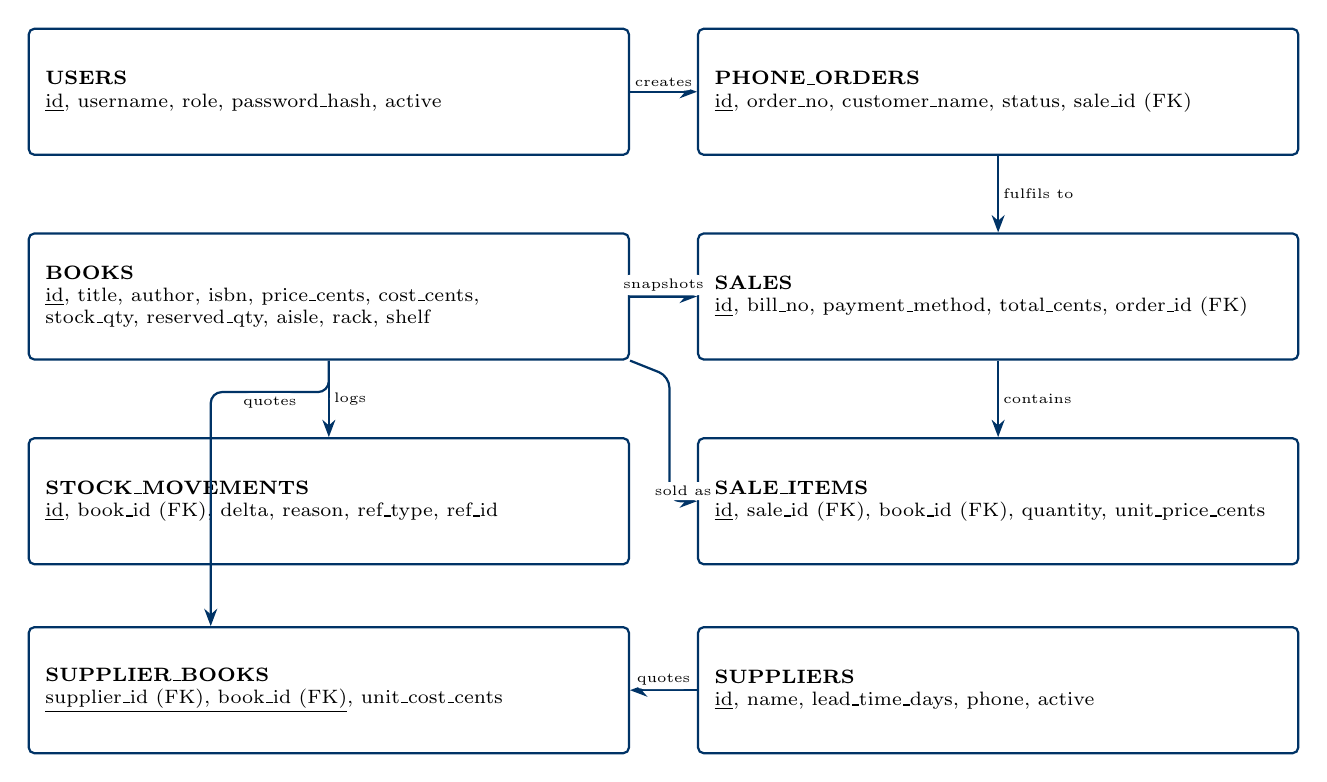
\begin{tikzpicture}[
    entity/.style={box, text width=7.2cm, minimum height=1.6cm, align=left},
    conn/.style={arrow, rounded corners=4pt}
]
    % Column 1
    \node[entity] (users) at (0, 7.0) {\textbf{USERS}\\\scriptsize \underline{id}, username, role, password\_hash, active};
    \node[entity] (books) at (0, 4.4) {\textbf{BOOKS}\\\scriptsize \underline{id}, title, author, isbn, price\_cents, cost\_cents,\\stock\_qty, reserved\_qty, aisle, rack, shelf};
    \node[entity] (movements) at (0, 1.8) {\textbf{STOCK\_MOVEMENTS}\\\scriptsize \underline{id}, book\_id (FK), delta, reason, ref\_type, ref\_id};
    \node[entity] (suppbooks) at (0, -0.6) {\textbf{SUPPLIER\_BOOKS}\\\scriptsize \underline{supplier\_id (FK), book\_id (FK)}, unit\_cost\_cents};

    % Column 2
    \node[entity] (orders) at (8.5, 7.0) {\textbf{PHONE\_ORDERS}\\\scriptsize \underline{id}, order\_no, customer\_name, status, sale\_id (FK)};
    \node[entity] (sales) at (8.5, 4.4) {\textbf{SALES}\\\scriptsize \underline{id}, bill\_no, payment\_method, total\_cents, order\_id (FK)};
    \node[entity] (sitems) at (8.5, 1.8) {\textbf{SALE\_ITEMS}\\\scriptsize \underline{id}, sale\_id (FK), book\_id (FK), quantity, unit\_price\_cents};
    \node[entity] (suppliers) at (8.5, -0.6) {\textbf{SUPPLIERS}\\\scriptsize \underline{id}, name, lead\_time\_days, phone, active};

    % Clean Connections
    \draw[conn] (users.east) -- node[lbl, above]{creates} (orders.west);
    \draw[conn] (books.east) -- node[lbl, above]{snapshots} (sales.west);
    \draw[conn] (sales.south) -- node[lbl, right]{contains} (sitems.north);
    \draw[conn] (books.south) -- node[lbl, right]{logs} (movements.north);
    \draw[conn] (books.south) -- ++(0,-0.4) -| node[lbl, near start, below]{quotes} ($(suppbooks.north)+(-1.5,0)$);
    \draw[conn] (suppliers.west) -- node[lbl, above]{quotes} (suppbooks.east);
    \draw[conn] (orders.south) -- node[lbl, right]{fulfils to} (sales.north);
    \draw[conn] (books.south east) -- ++(0.5,-0.2) |- node[lbl, near end, above]{sold as} (sitems.west);
\end{tikzpicture}
\caption{Relational entity-relationship model illustrating referential integrity constraints}
\label{fig:data_model}
\end{figure}

\section{Semantic Integrity Constraints}
\begin{itemize}[leftmargin=1.5em]
  \item \textbf{Stock Invariants \& Safety Reserves:} Physical stock counts must satisfy $\texttt{stock\_qty} \ge 0$. Furthermore, customer reservations must never exceed physical availability: $\texttt{reserved\_qty} \le \texttt{stock\_qty}$. Net sellable stock is evaluated on-the-fly as $\texttt{available} = \texttt{stock\_qty} - \texttt{reserved\_qty}$.
  \item \textbf{Fixed-Point Currency Standardization:} All financial computations use integer minor units (paise/cents) to eradicate binary floating-point drift. Percentages (discounts and taxes) are stored as basis points ($1\% = 100\,\text{bp}$).
  \item \textbf{Non-Destructive Audit History:} Deletion of sales or stock histories is strictly forbidden. Corrections flip record statuses to \texttt{voided} and issue compensatory entries within \texttt{stock\_movements}.
\end{itemize}

%============================================================
% FORCE ARCHITECTURE ON A SINGLE NEW PAGE
%============================================================
\clearpage
\chapter{System Architecture \& Subsystem Decomposition}
%============================================================
The system architecture follows a decoupled, four-tier model that establishes strict operational boundaries between client interactions, security verification, business domain processing, and transactional persistence.

\begin{figure}[H]
\centering
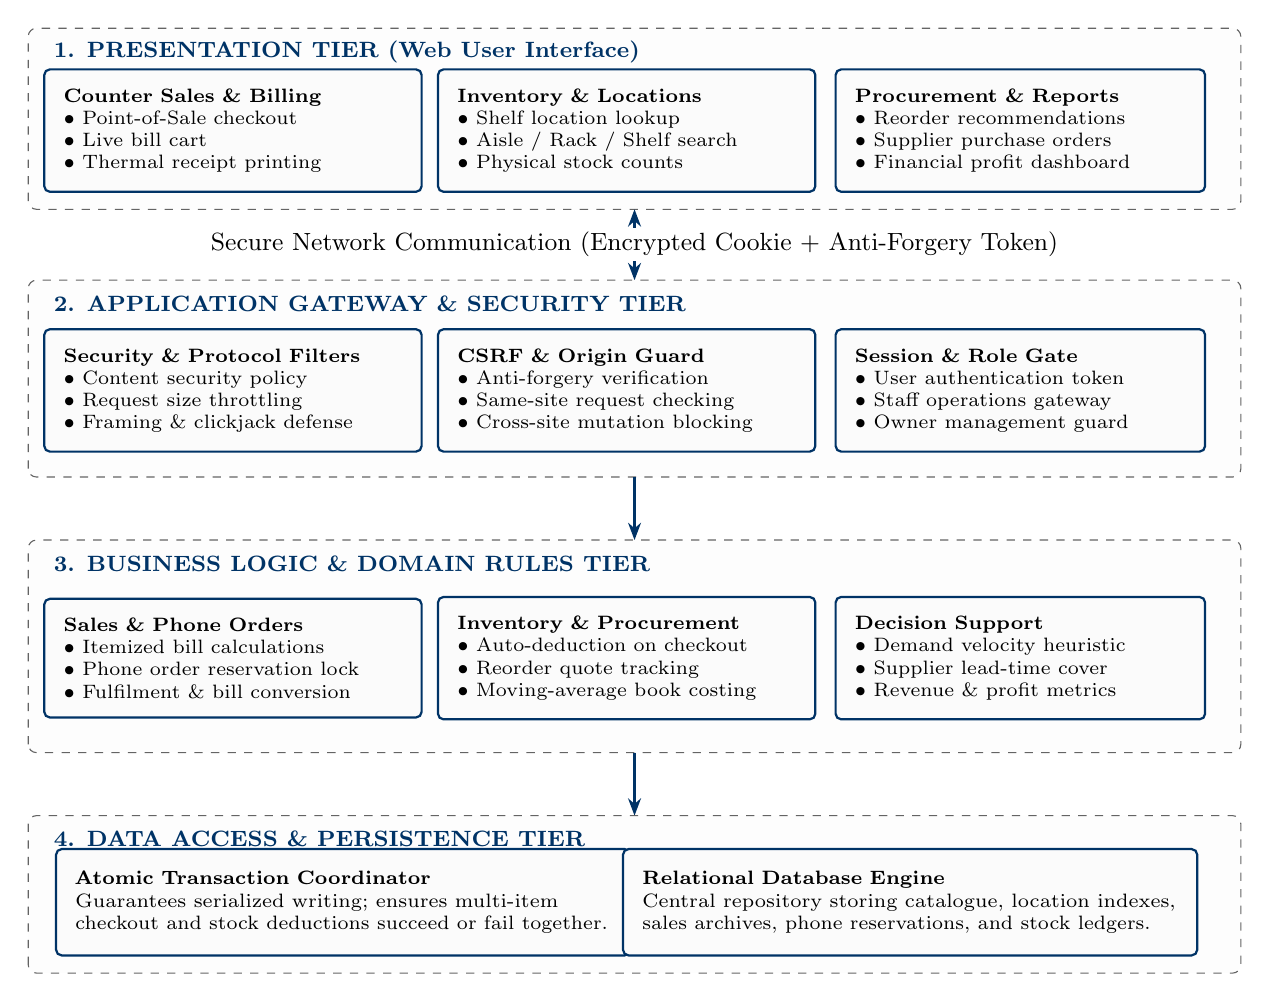
\begin{tikzpicture}[
    labelnode/.style={font=\bfseries\footnotesize\color{vjtiblue}, anchor=west}
]
    % Outer Frame 1: Presentation Layer
    \draw[wireframe] (-0.2, 7.7) rectangle (15.2, 10.0);
    \node[labelnode] at (0.0, 9.7) {1. PRESENTATION TIER (Web User Interface)};
    \node[paddedsubsys, text width=4.3cm] at (2.4, 8.7) {\textbf{Counter Sales \& Billing}\\\scriptsize $\bullet$ Point-of-Sale checkout\\\scriptsize $\bullet$ Live bill cart\\\scriptsize $\bullet$ Thermal receipt printing};
    \node[paddedsubsys, text width=4.3cm] at (7.4, 8.7) {\textbf{Inventory \& Locations}\\\scriptsize $\bullet$ Shelf location lookup\\\scriptsize $\bullet$ Aisle / Rack / Shelf search\\\scriptsize $\bullet$ Physical stock counts};
    \node[paddedsubsys, text width=4.2cm] at (12.4, 8.7) {\textbf{Procurement \& Reports}\\\scriptsize $\bullet$ Reorder recommendations\\\scriptsize $\bullet$ Supplier purchase orders\\\scriptsize $\bullet$ Financial profit dashboard};

    % Bridge Arrow
    \draw[darrow] (7.5, 7.7) -- node[lbl, fill=white]{\small Secure Network Communication (Encrypted Cookie + Anti-Forgery Token)} (7.5, 6.8);

    % Outer Frame 2: Gateway & Security Layer
    \draw[wireframe] (-0.2, 4.3) rectangle (15.2, 6.8);
    \node[labelnode] at (0.0, 6.5) {2. APPLICATION GATEWAY \& SECURITY TIER};
    \node[paddedsubsys, text width=4.3cm] at (2.4, 5.4) {\textbf{Security \& Protocol Filters}\\\scriptsize $\bullet$ Content security policy\\\scriptsize $\bullet$ Request size throttling\\\scriptsize $\bullet$ Framing \& clickjack defense};
    \node[paddedsubsys, text width=4.3cm] at (7.4, 5.4) {\textbf{CSRF \& Origin Guard}\\\scriptsize $\bullet$ Anti-forgery verification\\\scriptsize $\bullet$ Same-site request checking\\\scriptsize $\bullet$ Cross-site mutation blocking};
    \node[paddedsubsys, text width=4.2cm] at (12.4, 5.4) {\textbf{Session \& Role Gate}\\\scriptsize $\bullet$ User authentication token\\\scriptsize $\bullet$ Staff operations gateway\\\scriptsize $\bullet$ Owner management guard};

    % Arrow to Business Rules
    \draw[arrow] (7.5, 4.3) -- (7.5, 3.5);

    % Outer Frame 3: Business Logic Layer
    \draw[wireframe] (-0.2, 0.8) rectangle (15.2, 3.5);
    \node[labelnode] at (0.0, 3.2) {3. BUSINESS LOGIC \& DOMAIN RULES TIER};
    \node[paddedsubsys, text width=4.3cm] at (2.4, 2.0) {\textbf{Sales \& Phone Orders}\\\scriptsize $\bullet$ Itemized bill calculations\\\scriptsize $\bullet$ Phone order reservation lock\\\scriptsize $\bullet$ Fulfilment \& bill conversion};
    \node[paddedsubsys, text width=4.3cm] at (7.4, 2.0) {\textbf{Inventory \& Procurement}\\\scriptsize $\bullet$ Auto-deduction on checkout\\\scriptsize $\bullet$ Reorder quote tracking\\\scriptsize $\bullet$ Moving-average book costing};
    \node[paddedsubsys, text width=4.2cm] at (12.4, 2.0) {\textbf{Decision Support}\\\scriptsize $\bullet$ Demand velocity heuristic\\\scriptsize $\bullet$ Supplier lead-time cover\\\scriptsize $\bullet$ Revenue \& profit metrics};

    % Arrow to Data Access
    \draw[arrow] (7.5, 0.8) -- (7.5, 0.0);

    % Outer Frame 4: Data Persistence Layer
    \draw[wireframe] (-0.2, -2.0) rectangle (15.2, 0.0);
    \node[labelnode] at (0.0, -0.3) {4. DATA ACCESS \& PERSISTENCE TIER};
    \node[paddedsubsys, text width=6.8cm] at (3.8, -1.1) {\textbf{Atomic Transaction Coordinator}\\\scriptsize Guarantees serialized writing; ensures multi-item checkout and stock deductions succeed or fail together.};
    \node[paddedsubsys, text width=6.8cm] at (11.0, -1.1) {\textbf{Relational Database Engine}\\\scriptsize Central repository storing catalogue, location indexes, sales archives, phone reservations, and stock ledgers.};
\end{tikzpicture}
\caption{Four-tier functional architecture diagram with enhanced submodule padding}
\label{fig:high_level_arch}
\end{figure}

\section{Tiered Responsibilities \& Capability Partitioning}
Table~\ref{tab:layers} outlines the functional partitioning across the four architectural boundaries.

\begin{table}[H]
\centering
\footnotesize
\begin{tabularx}{\textwidth}{L{3.5cm} L{6.0cm} L{5.9cm}}
\toprule
\textbf{Architectural Tier} & \textbf{Core Purpose} & \textbf{Key Capabilities Provided} \\
\midrule
Presentation Tier & Delivers responsive screens and captures operator keystrokes/scans. & Point-of-Sale checkout, shelf location lookup, phone order queue, owner reports. \\
Gateway Tier & Sanitizes transport payloads and verifies user identities. & Header inspection, anti-forgery verification, role-based boundary control. \\
Business Logic Tier & Executes domain workflows, mathematical pricing, and restocking logic. & Tax and discount calculation, reservation holds, demand velocity ranking. \\
Persistence Tier & Coordinates concurrent writes and guarantees durability. & Serialized write locking, relational storage, append-only movement logs. \\
\bottomrule
\end{tabularx}
\caption{Architectural tiers, functional scopes, and provided capabilities}
\label{tab:layers}
\end{table}

\section{Key Architectural Tenets}
\begin{itemize}[leftmargin=1.5em]
  \item \textbf{Single Source of Business Truth:} The client interface serves as an input/output terminal; all pricing arithmetic, stock availability checks, and status mutations are enforced exclusively on the backend.
  \item \textbf{Atomic Multi-Record Mutations:} Any checkout or fulfillment involves concurrent updates across sales, lines, and stock ledgers. These operate under exclusive write locks, rolling back completely if any single constraint fails.
  \item \textbf{Privileged Information Isolation:} Wholesale book costs, vendor margins, and net profit calculations are inaccessible to counter staff, safeguarding sensitive financial metrics.
\end{itemize}

%============================================================
\chapter{Data Flow Analysis \& Transform Mapping}
%============================================================
Transform mapping models computational workflows where continuous inputs are assembled, transformed within a central decision module, and emitted as permanent artifacts. Figure~\ref{fig:transform} depicts the **Point-of-Sale Counter Billing Pipeline**.

\begin{figure}[H]
\centering
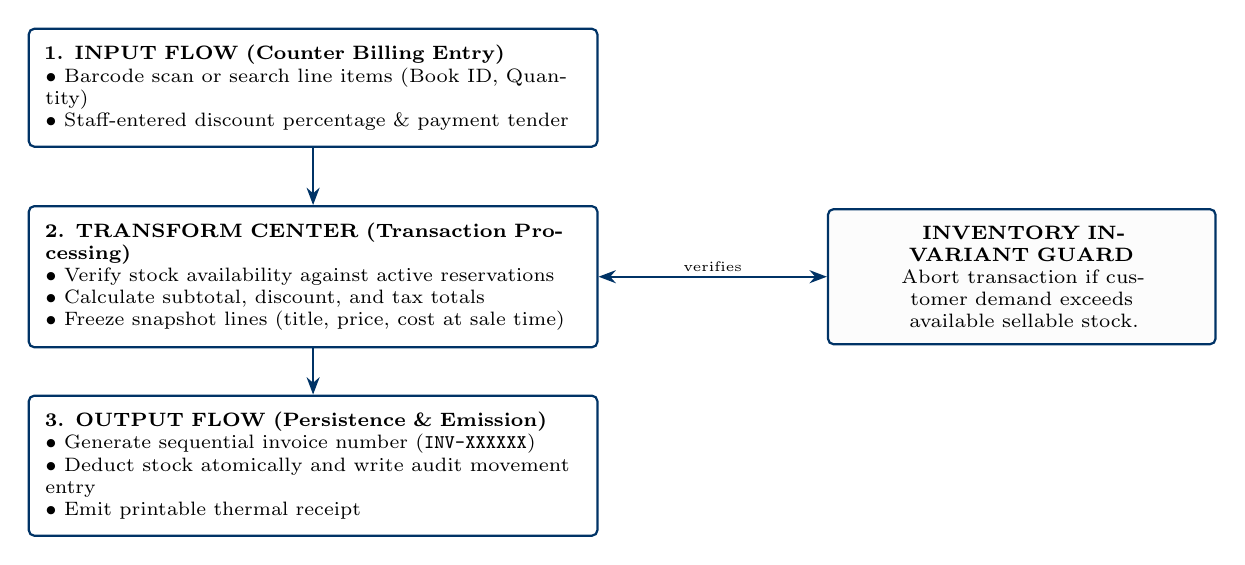
\begin{tikzpicture}[
    tbox/.style={box, text width=6.8cm, minimum height=1.3cm, align=left},
    arr/.style={arrow, rounded corners=3pt}
]
    % Main vertical sequence
    \node[tbox] (inflow) at (0, 5.0) {
        \textbf{1. INPUT FLOW (Counter Billing Entry)}\\
        \scriptsize $\bullet$ Barcode scan or search line items (Book ID, Quantity)\\
        \scriptsize $\bullet$ Staff-entered discount percentage \& payment tender
    };

    \node[tbox] (transform) at (0, 2.6) {
        \textbf{2. TRANSFORM CENTER (Transaction Processing)}\\
        \scriptsize $\bullet$ Verify stock availability against active reservations\\
        \scriptsize $\bullet$ Calculate subtotal, discount, and tax totals\\
        \scriptsize $\bullet$ Freeze snapshot lines (title, price, cost at sale time)
    };

    \node[tbox] (outflow) at (0, 0.2) {
        \textbf{3. OUTPUT FLOW (Persistence \& Emission)}\\
        \scriptsize $\bullet$ Generate sequential invoice number (\texttt{INV-XXXXXX})\\
        \scriptsize $\bullet$ Deduct stock atomically and write audit movement entry\\
        \scriptsize $\bullet$ Emit printable thermal receipt
    };

    % Invariant side check
    \node[box, text width=4.5cm, fill=lightgray!30] (guard) at (9.0, 2.6) {
        \textbf{INVENTORY INVARIANT GUARD}\\
        \scriptsize Abort transaction if customer demand exceeds available sellable stock.
    };

    \draw[arr] (inflow) -- (transform);
    \draw[arr] (transform) -- (outflow);
    \draw[darrow] (transform) -- node[lbl, above]{verifies} (guard);
\end{tikzpicture}
\caption{Transform mapping for the Point-of-Sale counter checkout process}
\label{fig:transform}
\end{figure}

\section{Pipeline Derivation Methodology}
\begin{enumerate}[leftmargin=1.5em]
  \item \textbf{Ingestion Phase:} Line items, quantities, and discount requests are collected at the counter terminal and checked for structural validity.
  \item \textbf{Transformation Center:} The processor fetches catalog prices, asserts availability against active telephone reservations, computes financial net totals in integer basis points, and locks unit costs into line snapshots.
  \item \textbf{Emission Phase:} An invoice sequence number is issued, inventory counts are decremented, immutable ledger records are recorded, and a receipt summary is returned for thermal printing.
\end{enumerate}

%============================================================
\chapter{Operational Dispatching \& Transaction Mapping}
%============================================================
Transaction mapping structures systems where incoming operational triggers are categorized by an evaluation node and routed along mutually exclusive execution channels. Figure~\ref{fig:transaction} models the **Operational Request Dispatcher**.

\begin{figure}[H]
\centering
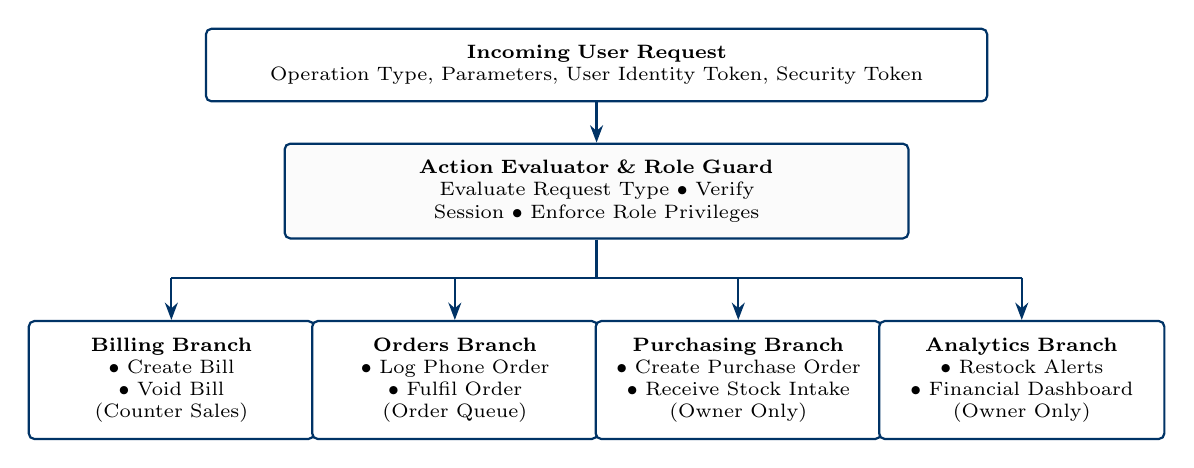
\begin{tikzpicture}[
    arr/.style={arrow, rounded corners=4pt}
]
    % Root Request
    \node[box, text width=9.5cm] (req) at (0, 4.8) {
        \textbf{Incoming User Request}\\\scriptsize Operation Type, Parameters, User Identity Token, Security Token
    };

    % Evaluator
    \node[box, text width=7.5cm, fill=lightgray!40] (eval) at (0, 3.2) {
        \textbf{Action Evaluator \& Role Guard}\\\scriptsize Evaluate Request Type $\bullet$ Verify Session $\bullet$ Enforce Role Privileges
    };

    % 4 Action Branches
    \node[box, text width=3.2cm] (b1) at (-5.4, 0.8) {
        \textbf{Billing Branch}\\\scriptsize $\bullet$ Create Bill\\\scriptsize $\bullet$ Void Bill\\\scriptsize (Counter Sales)
    };
    \node[box, text width=3.2cm] (b2) at (-1.8, 0.8) {
        \textbf{Orders Branch}\\\scriptsize $\bullet$ Log Phone Order\\\scriptsize $\bullet$ Fulfil Order\\\scriptsize (Order Queue)
    };
    \node[box, text width=3.2cm] (b3) at (1.8, 0.8) {
        \textbf{Purchasing Branch}\\\scriptsize $\bullet$ Create Purchase Order\\\scriptsize $\bullet$ Receive Stock Intake\\\scriptsize (Owner Only)
    };
    \node[box, text width=3.2cm] (b4) at (5.4, 0.8) {
        \textbf{Analytics Branch}\\\scriptsize $\bullet$ Restock Alerts\\\scriptsize $\bullet$ Financial Dashboard\\\scriptsize (Owner Only)
    };

    % Orthogonal Dispatch Bus
    \draw[arr] (req) -- (eval);
    \draw[thick, vjtiblue] (eval.south) -- (0, 2.1);
    \draw[thick, vjtiblue] (-5.4, 2.1) -- (5.4, 2.1);

    \draw[arr] (-5.4, 2.1) -- (b1.north);
    \draw[arr] (-1.8, 2.1) -- (b2.north);
    \draw[arr] (1.8, 2.1) -- (b3.north);
    \draw[arr] (5.4, 2.1) -- (b4.north);
\end{tikzpicture}
\caption{Transaction mapping tree for request routing and role authorization}
\label{fig:transaction}
\end{figure}

\section{Route Execution Channels}
\begin{itemize}[leftmargin=1.5em]
  \item \textbf{Counter Checkout Channel:} Manages cashier retail transactions, checks discount authorizations, and coordinates atomic stock write-offs.
  \item \textbf{Telephone Orders Channel:} Oversees order intake, manages stock reservation holds, and handles balance settlement upon order delivery.
  \item \textbf{Purchasing \& Intake Channel (Owner):} Coordinates replenishment purchase orders with vendors and re-averages acquisition costs upon goods arrival.
  \item \textbf{Business Intelligence Channel (Owner):} Generates velocity-based reorder notifications and compiles net profit summaries.
\end{itemize}

%============================================================
\chapter{Interaction Design \& User Experience Principles}
%============================================================
The user interface adheres to a utilitarian, ledger-centric visual language. The design emphasizes immediate legibility, high contrast, monospaced numerical tables, and keyboard ergonomics over decorative visual elements.

\section{Interface Elements \& Ergonomics}
\begin{table}[H]
\centering
\footnotesize
\begin{tabularx}{\textwidth}{L{3.8cm} L{11.4cm}}
\toprule
\textbf{Interaction Element} & \textbf{Ergonomic \& Operational Role} \\
\midrule
Role-Gated Sidebar & Organizes navigation by domain (Sales, Stock, Intelligence, System), automatically hiding privileged owner tabs from counter staff. \\
Split-Pane POS Console & Divides the counter screen into a catalog lookup area on the left and an active checkout ledger on the right for seamless line adjustments. \\
Scanner Emulation Pickup & Directly binds to standard USB barcode readers, immediately adding titles to the active cart upon scanning an ISBN. \\
Re-entrance Protection & Wraps action buttons in a client-side execution lock, preventing accidental duplicate form submissions from rapid double-clicking. \\
Print-Media Receipt Modal & Renders an itemized paper receipt optimized for standard thermal slip printers, omitting visual navigation elements. \\
\bottomrule
\end{tabularx}
\caption{User interface components and operational design characteristics}
\label{tab:ui_elements}
\end{table}

\section{Operator Usability Guidelines}
\begin{itemize}[leftmargin=1.5em]
  \item \textbf{Frictionless Keystroke Flow:} Key search bars autofocus on load, allowing sales clerks to search, add, discount, and tender bills without using the mouse.
  \item \textbf{Immediate Stock Visibility:} Cart items surface active stock counts and warning badges if requested quantities approach shelf thresholds.
  \item \textbf{High-Impact Confirmation:} Destructive actions, such as voiding finalized bills or manual stock overrides, mandate explicit operator reason codes.
\end{itemize}

%============================================================
\chapter{Detailed Algorithmic \& Component Specifications}
%============================================================
Procedural design formalizes the internal decision structures, validation checkpoints, and computational routines governing domain operations.

\section{Checkout Workflow Execution (Flowchart)}
Figure~\ref{fig:flowchart} outlines the procedural flow of the checkout execution logic, detailing the invariant validation branch.

\begin{figure}[H]
\centering
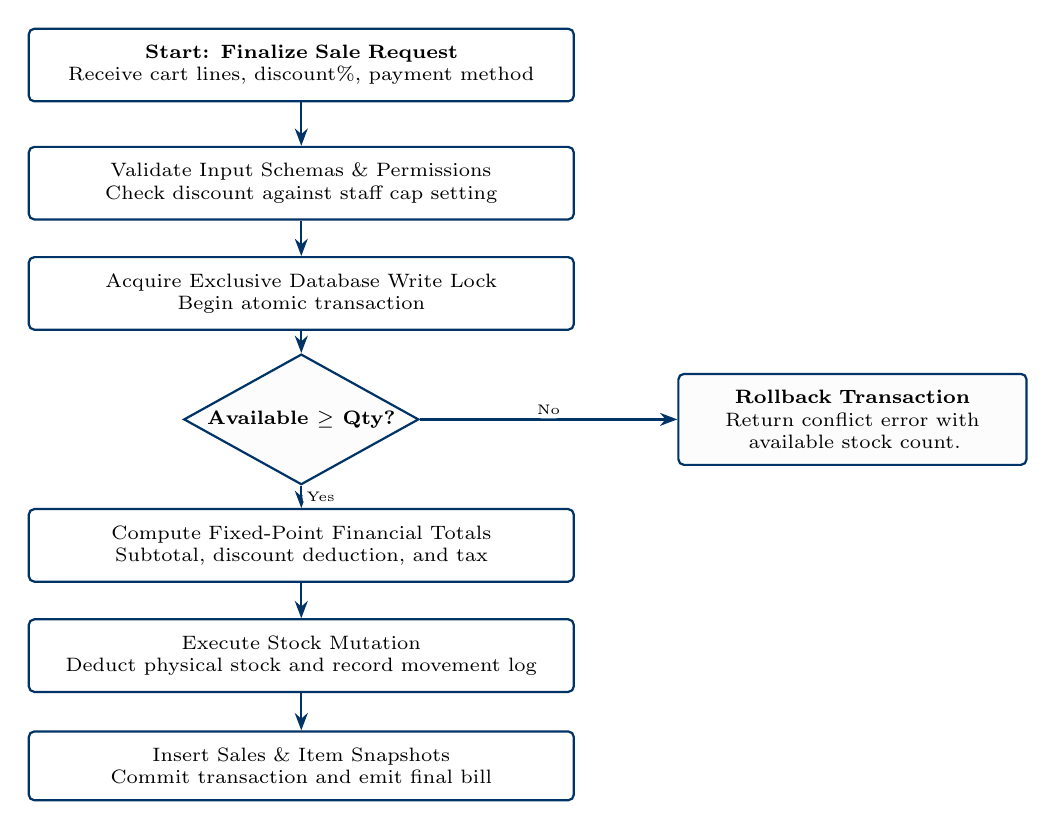
\begin{tikzpicture}[
    fnode/.style={box, text width=6.5cm, align=center},
    arr/.style={arrow, rounded corners=3pt}
]
    \node[fnode] (start) at (0, 7.5) {\textbf{Start: Finalize Sale Request}\\\scriptsize Receive cart lines, discount\%, payment method};
    \node[fnode] (val) at (0, 6.0) {Validate Input Schemas \& Permissions\\\scriptsize Check discount against staff cap setting};
    \node[fnode] (lock) at (0, 4.6) {Acquire Exclusive Database Write Lock\\\scriptsize Begin atomic transaction};
    \node[decision] (dec) at (0, 3.0) {\scriptsize Available $\ge$ Qty?};
    \node[fnode] (calc) at (0, 1.4) {Compute Fixed-Point Financial Totals\\\scriptsize Subtotal, discount deduction, and tax};
    \node[fnode] (stock) at (0, 0.0) {Execute Stock Mutation\\\scriptsize Deduct physical stock and record movement log};
    \node[fnode] (save) at (0, -1.4) {Insert Sales \& Item Snapshots\\\scriptsize Commit transaction and emit final bill};

    % Error node
    \node[box, text width=4.0cm, fill=lightgray!30] (err) at (7.0, 3.0) {
        \textbf{Rollback Transaction}\\\scriptsize Return conflict error with available stock count.
    };

    % Connections
    \draw[arr] (start) -- (val);
    \draw[arr] (val) -- (lock);
    \draw[arr] (lock) -- (dec);
    \draw[arr] (dec) -- node[lbl, right]{Yes} (calc);
    \draw[arr] (calc) -- (stock);
    \draw[arr] (stock) -- (save);
    \draw[arr] (dec) -- node[lbl, above]{No} (err);
\end{tikzpicture}
\caption{Procedural decision flowchart for checkout validation and inventory deduction}
\label{fig:flowchart}
\end{figure}

\section{Algorithmic Logic: Reorder Prioritization Heuristic}
The restocking recommendation system computes reorder suggestions based on empirical sales velocity, existing reservations, incoming shipments, and supplier delivery windows.

\begin{lstlisting}[language=Python, caption={Algorithmic Pseudocode for Empirical Restocking Analysis}]
PROCEDURE CalculateRestockPriorities(analysisWindowDays, targetCoverageDays):
    systemConfig <- LoadStoreParameters()
    window <- DefaultIfNull(analysisWindowDays, systemConfig.defaultWindow)
    coverage <- DefaultIfNull(targetCoverageDays, systemConfig.defaultCoverage)
    
    catalogTitles <- RetrieveActiveBookCatalog()
    historicalSales <- AggregateSalesByTitle(timeframeDays = window)
    pendingShipments <- AggregateUnitsOnOpenOrders()
    
    reorderMatrix <- []
    
    FOR EACH book IN catalogTitles:
        quantitySold <- historicalSales.get(book.id, 0)
        daysTracked <- (SystemDate() - book.catalogDate).days
        observedDays <- Clamp(daysTracked, min = 1, max = window)
        
        salesVelocity <- quantitySold / observedDays
        availableInventory <- book.stockQty - book.reservedQty
        pipelineInventory <- pendingShipments.get(book.id, 0)
        safetyThreshold <- DefaultIfNull(book.minThreshold, systemConfig.defaultThreshold)
        
        leadTimeDays <- FetchFastestSupplierLeadTime(book.id, fallback = systemConfig.defaultLead)
        daysOfSupply <- (availableInventory / salesVelocity) IF salesVelocity > 0 ELSE Infinity
        
        urgencyRank <- NULL
        justificationList <- []
        
        IF quantitySold > 0 AND availableInventory <= 0:
            urgencyRank <- "CRITICAL"
            justificationList.append("Depleted inventory with sustained sales velocity")
        ELSE IF salesVelocity > 0 AND daysOfSupply < leadTimeDays:
            urgencyRank <- "HIGH"
            justificationList.append("Imminent stockout: supply runs out before reorder arrives")
        ELSE IF availableInventory <= safetyThreshold AND (availableInventory + pipelineInventory) <= safetyThreshold:
            urgencyRank <- "MEDIUM"
            justificationList.append("Inventory breached minimum safety reserve")
        END IF
        
        IF urgencyRank IS NOT NULL:
            targetBuffer <- Ceil(salesVelocity * coverage) + safetyThreshold
            recommendedReorder <- Max(1, targetBuffer - (availableInventory + pipelineInventory))
            primarySupplier <- FetchCheapestSupplier(book.id)
            
            reorderMatrix.append({
                id: book.id,
                title: book.title,
                urgency: urgencyRank,
                reorderUnits: recommendedReorder,
                estimatedExpenditure: recommendedReorder * primarySupplier.quotedPrice
            })
        END IF
    END FOR
    
    RETURN SortByUrgencyDescending(reorderMatrix)
END PROCEDURE
\end{lstlisting}

%============================================================
\chapter{Functional Scope Verification}
%============================================================
Table~\ref{tab:req_mapping} validates that all seven functional requirements from Assignment 1 are supported by explicit architectural constructs.

\begin{table}[H]
\centering
\footnotesize
\begin{tabularx}{\textwidth}{L{4.2cm} L{11cm}}
\toprule
\textbf{Functional Requirement} & \textbf{Architectural \& Procedural Realization} \\
\midrule
4.1 Shelf Coordinates \& Master Catalog & Relational schema incorporating Aisle, Rack, and Shelf coordinates, backed by multi-attribute indexing and search parsers. \\
4.2 Point-of-Sale Billing Console & Transform-mapped checkout pipeline, integer minor unit arithmetic, and scanner-friendly UI panes. \\
4.3 Automated Stock Deduction & Atomic guarded updates, append-only chronological movement ledgers, and database invariants. \\
4.4 Empirical Restocking Analytics & Procedural velocity-over-lead-time algorithms surfacing prioritized reorder suggestions. \\
4.5 Distributor Management & Vendor quote tracking, Purchase Order lifecycle management, and goods receipt intake reconciler. \\
4.6 Consolidated Financial Dashboard & Multi-period aggregation queries for Net Revenue, COGS, Operating Overhead, and Gross Profit. \\
4.7 Telephone Order Management & Stateful lifecycle model (Intake to Fulfilled) with stock reservation holds and signed payment ledgers. \\
\bottomrule
\end{tabularx}
\caption{Traceability matrix connecting functional requirements to design specifications}
\label{tab:req_mapping}
\end{table}

%============================================================
\chapter{Deliverables Summary \& Concluding Remarks}
%============================================================
\section{Engineering Deliverables Checklist}
\begin{itemize}[leftmargin=1.5em]
  \item Fully normalized logical entity catalog with referential constraints, stock invariants, and minor-unit financial rules.
  \item A comprehensive four-tier architectural decomposition with enhanced submodule breathing room and padding.
  \item Linear transform mapping pipeline modeling the checkout workflow.
  \item Operational transaction mapping tree categorizing request types and enforcing role permissions.
  \item Interaction design specifications optimized for retail cashiering.
  \item Formal decision flowcharts and pseudocode algorithms for stock synchronization and empirical restocking heuristics.
  \item Traceability verification matrix confirming complete coverage of functional commitments.
\end{itemize}

\section{Concluding Remarks}
The design models formulated in this specification establish a complete, verified engineering foundation for the Bookshop Automation System. By relying on atomic write locks, strict reservation holds, append-only ledgers, and decoupled role-based security barriers, the system ensures data consistency and mathematical reliability across all retail operations.

\end{document}

